% !TEX root = ../main.tex

\chapter{Related Work}
\label{chapter:RelWork}
Our work focuses on learning a policy to solve POMDPs where only a single observation is given. We assume some expert demonstrations and the access to a sparse 
reward of wether the task was successfully solved. While to the authors knowledge, there is no approach specifically tailored for this setup, 
in this chapter we will cover approaches that aim to solve aspects of the given setup.

\section{Sparse Reward}
Learning with sparse rewards is challenging in a high dimensional action and observation space, as nearly all trajectories will have reward 0. 
Until by chance a succesful trajectory is found, the agent has to blindly guess. To overcome this problem, Marcin Andrychowicz et. al propose 
"Hindsight Experience Replay".

The algorithm works by generating new goals for a given trajectory based on the states that were actually reached. 
Specifically, consider the problem of finding a policy $\pi(a|o, g)$ given observation $o$ and goal $g$. 
If the goal is reached, the reward is 1. Given a state at time step t $s_t$ and a goal state g, with $s_t != g$, 
the reward for the state is $r(s_t|g) = 0$, which does not provide much information for the policy. 
To use the information of which state was actually
reached by the trajectory, a new goal is constructed $g' = s_t$. Using this, the new reward is $r(s_t|g') = 1$. 
The agent can then learn from these hindsight goals, which can provide more 
frequent rewards and enable faster learning. An additional advantage of HER is that it is agnostic with respect to the learning algorithm, as it only 
provides additional trajectories for the replay buffer.\\

Overall, HER is a powerful algorithm that addresses the problem of sparse rewards in reinforcement learning by leveraging hindsight. It has been successfully 
applied to a wide range of tasks, including robotic manipulation, locomotion, and game playing, and has shown superior performance compared to standard 
reinforcement learning algorithms.\\
A downside of HER is, that it requires the inverse function $g(s)$, meaning from a visited state, the goal must be reconstructable. This is not always given. 
Consider the goal of not driving into a vehicle or a goal expressed in natural language. 

Reinforcement Learning with Sparse Rewards using Guidance from Offline Demonstration - 

-needs partially leared expert to aim training
https://arxiv.org/abs/2202.04628 

\section{Single Observation Imitation Learning in POMDPs}
\label{LCILRM}
The paper "Language-Conditioned Imitation Learning for Robot Manipulation Tasks" \cite{stepputtis2020languageconditioned} proposes a method for robot manipulation tasks that takes 
into account natural language instructions. The proposed method involves using a neural network to map natural language instructions to 
corresponding robot actions. The authors also introduce a novel dataset of language-conditioned robot manipulation tasks, which they use to evaluate 
their method. The experimental results demonstrate the effectiveness of their approach in inferring and executing trajectories for robot manipulation 
tasks when language instructions are given.\\

A policy $\pi(v,I)$ is learned to imitate expert behavior in a set of demonstrations $D = \{d_0,...,d_m\}$, each containing a trajectory 
$R \in R^{T \times N}$ over $T$ time steps and with $N$ control variables, an rgb image $I \in \mathcal{R}^{569 \times 320 \times 3}$ of the agent's surroundings, 
and a task description $v \in \mathcal{R}^{15 \times 50}$ from natural language using GloVe \cite{pennington-etal-2014-glove} embeddings. The proposed method takes the image $I$ and task description $v$ 
to create a task embedding $e$ using GloVe embeddings and a pretrained image recognition model in the semantic model, 
which is subsequently used in the control model to generate robot actions at each time in a closed-loop 
fashion. A schematic overview can be seen in figure \ref{language_imitation}.

Crucially, there is only one observation per trajectory, so we have a POMDP, where we only know the state of the system at time point $t=0$. In this paper, the 
algorithm uses a GRU to ceep track of the former history of the POMDP, similar to the approach described in \ref{POMDP_RNN}. In addition to the hidden state, 
the task embedding $e$ is used in every timestep, as we know, that the task does not change. \\

\begin{figure}[htbp]
    \centering
    \includegraphics[width=\textwidth]{images/Language_Conditioned/System.pdf}
    \caption{Overview of the general system architecture. (Left) Details of the controller model, which
    synthesizes robot control signals . (Right) details of the semantic model, which extracts critical
    information about the task from both perceptual input and language commands. Dark-blue boxes
    indicate pre-trained components of the model \cite{stepputtis2020languageconditioned}.}
    \label{language_imitation}
\end{figure}

The learned behaviour consists of picking up objects and pouring their content into other objects. First, a sentense in natural language describes the object, which 
the agent should pick up. For example "Pick up the red cup". This command in combination with the rgb image of the scene is used to generate the trajectory to 
pick up the cup. Then an object is described, into which the robot should pour the content. For example "Pour some of it into the blue bowl". An overview over 
all possible objects and the described example can be found in figure \ref{lang_imi_expl}. The dataset consists of 45 000 tasks, where 4000 tasks are used for 
evaluation and 1000 tasks are used for testing. The authors find that their model can perform $98 \%$ of pick tasks, $85 \%$ of pour tasks and $84 \%$ combined 
tasks, which greatly outperforms a baseline using an end to end RNN model with $58\%$ success rate for picking and $0 \%$ success rate for pouring.

\begin{figure}[htbp]
    \centering
    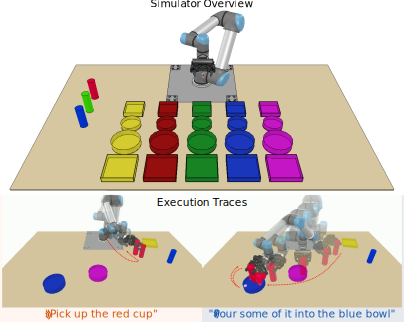
\includegraphics[width=\textwidth]{images/Language_Conditioned/simulator.pdf}
    \caption{Overview of a task. (top) - All possible objects and colors. (left) Example trajectory to "pick up the red cup" following the natural language description. 
    (right) Example trajectory to "pour some of it into the blue bowl". Figure taken from \cite{stepputtis2020languageconditioned}.}
    \label{lang_imi_expl}
\end{figure}

\section{Fine Tuning with Sparse Rewards}
Fine-tuning in RL refers to the process of adapting a pre-trained RL model to a new task or environment. In this thesis, fine tuning is done by using behavioural 
cloning on an expert dataset with n trajectories. In the fine tuning phase, the pretrained policy is used in the environment of the task and adiitional feedback 
like sparese rewards are used to enhance the performance of the policy. Fine tuning is a common approach to overcome the exploration problem of high dimensional 
spaces.
\subsection{Sparse Rewards in MDPs with Expert Demonstrations}
In the paper Leveraging Demonstrations for Deep Reinforcement Learning on Robotics Problems with Sparse Rewards \cite{LDDRLP} the authors describe a priority 
sampling algorithm in combination with the deep deterministic policy gradient (DDPG) algorithm as described in \ref{AC-Alg}. The probability with which a 
training sample is chosen from the replay buffer is described as:
\begin{equation}
    P(i) = \frac{p_i^\alpha}{\sum\limits_{k} p_k^\alpha}
\end{equation}
with 
\begin{equation}
    p_i = \delta_{i}^2 + \lambda \lvert \nabla_a Q(s_i, a_i \vert \theta_Q) \rvert^2 + \epsilon + \epsilon_{D}.
\end{equation}
Here $\delta_{i}$ is the temporal difference error, $\lambda$ is used to weigh the importance of the sample i with respect to the loss of the actor, 
$\epsilon$ is a small constant to ensure every transition is chosen with probability $p_i > 0$ and $\epsilon_D$ is a positive constant aplied for expert transitions.\\
The idea behind this importance sampling algorithm is to amment the priority experience replay probability as developed in \cite{https://arxiv.org/pdf/1511.05952.pdf} 
with a constant $\epsilon_{D}$ for expert demonstrations to make the policy converge faster to the expert behaviour. In priority experience replay, more rare 
experiences are chosen more likely to use the data in the replay buffer more efficiently. Moreover, they use a combination between $n=1$ temporal difference and 
$n=N > 1$ temporal difference to get better estimations for rewards that are in the distant future, as they assume sparse rewards.\\
The effectiveness of the approach is demonstrated by comparing the performance of their importance sampling algorithm with sparse rewards to a standard DDPG 
implementation using no expert demonstration but dense reward. The authors find that their approach can learn faster then standard DDPG with 100 expert 
demonstrations on a challenging robotic insertion task.\\ 
A problem with this approach is, that the critic assumes the demporal difference error approximates the distribution induced by the policy $\pi_{\theta}$, but by 
mixing in expert demonstrations, the expected $Q$ value will be higher, then that of the policy $\pi_{\theta}$. This overestimation can lead to poor performance. 
The authors include a term to "weigh the update to the network" $w_i = \frac{1}{N} \cdot \frac{1}{P(i)}$. This term however is inversly proportinal to the 
probability of choosing a transition and thus counter acts the improvement rate towards expert behaviour.

\subsection{GAIL in POMDPs}
\label{GAIL_POMDPS}
Recall that GAIL optimized the objective
\begin{equation*}
    \min_{\theta} \max_{\omega} \mathbb{E}_{(s,a)\sim \pi_{\theta}, \mathcal{T}} [\log(1 - D_{\omega}(s,a))] + \mathbb{E}_{(s,a)\sim \mathcal{M}_{\text{E}}} [\log D_{\omega}(s,a)]
\end{equation*}
as derived in \ref{GAIL_Obj}, where $\mathbb{E}_{(s,a)\sim \mathcal{M}_{\text{E}}}$ denotes the expected distribution of the expert policy and 
$\mathbb{E}_{(s,a)\sim \pi, \mathcal{T}}$ denotes the expected distribution of the learned policy $\pi$, $D_{\omega}$ is the discriminator measuring how likely a state 
action pair was induced by the expert policy or the learned policy $\pi_{\theta}$. The paper "Learning Belief Representations for Imitation Learning in POMDPs" \cite{https://arxiv.org/pdf/1906.09510.pdf} 
extends the GAIL paradigm to work on POMDPs. To do so, they intorduce a network $B_{\phi}(o_{\leqt}, a_{\leqt}) = b_{t, \phi}$ that aims to approximate a 
representation of the beliefe state $b_t$ \ref{pomdp_bayes}, which forms a sufficient statistic for the POMDP 
$p(s_t|o_{\leq t}, a_{\leq t}) = p(s_t|b_t) \approx p(s_t|b_{t, \phi})$. Using $b_{\phi}$ instead of $s$ the new objective is:
\begin{equation}
    \min_{\phi,\theta}\max_{\tilde{\omega}} &\mathbb{E}_{(b,a)\sim\mathcal{M}_{\text{E}}}[\log D_{\tilde{\omega}}(b_{\phi},a)] + \mathbb{E}_{(b,a)\sim\pi,\mathcal{T}}[\log(1-D_{\tilde{\omega}}(b_{\phi},a))]
\end{equation}
with the correpsonding imitation loss 
$\mathcal{L}^{\text{IM}}(\phi) := D_{\text{JS}}(\theta,\phi) \approx \tilde{E}_{(h,a)\sim \mathcal{M}_\text{E}}[\log D^*(b_\phi(h),a)] + \tilde{E}_{(h,a)\sim \pi_\theta(a|b_\phi(h)),\mathcal{T}}[\log(1 - D^*(b_\phi(h),a))]$, 
where $D^*$ denotes the optimal discriminator. 
The authors include three regularisation losses to improve the expressiveness of $b_{\phi}$. For example:
\begin{equation}
    \mathcal{L}^f(\phi) = \mathbb{E}|| o_{t+k} - g(b_t^\phi, a_{t:t+k-1})||_2^2
\end{equation}
, where g is a learned stochastic unimodal gaussion with learned mean and fixed variance. Intuitively, this term seeks to impose, that the beliefe state $b_t$ is indeed a suffiecient statistic for the 
POMDP, by forcing the model $b_{\phi}$ to learn a representation that can predict future observations given future actions. The superscript $f$ of the regularisation loss means forward. 
In a similar way, there is an inverse regularisation $i$, which looks k steps into the past. Additionally, the authors propose an action regularisation $a$ which tries to reproduce the actions that were 
taken, given the initial beliefe state and the subsequent observations. With all three regularisation losses, the total loss function for the believe module is:
\begin{equation}
    L(\phi) = L^\text{IM} + \lambda_1 L^\text{f} + \lambda_2 L^\text{i} + \lambda_3 L^\text{a}
\end{equation}
, where $\lambda_i$ are the weights for the respective regularizors. \\
The approach is superior to GAIL with frame stacking and can also improve upon GAIL with recurrent networks for the discriminator and the actor, though the margins are small in some cases. The advantage 
of their approach is, that the believe state representation will be expressive following their regularizors. However, they use an l2 error between the predictions and the observations. In most environments, 
the observations are high dimensional and include redundant or unnecessary information that will be hard to learn. This forces the network to allocate capacity that is not directly used to 
optimize the overall objective. Moreover, as GAIL, this approach suffers from bad sample efficiency with respect to environment interactions.

\subsection{Mastering Atari, Go, Chess and Shogi by Planning with a
Learned Model}

In "Mastering Atari, Go, Chess and Shogi by Planning with a
Learned Model" \ref{MUZero}, the MuZero algorithm is derived. It is designed to achieve state-of-the-art performance 
in a wide range of games without any prior knowledge of the game rules, unlike its predecessor AlphaGo and AlphaZero, which relied on a hand-crafted 
domain-specific algorithm. MuZero learns to play games by combining deep neural networks with Monte Carlo tree search to plan and evaluate its actions. 
It does not have access to the game states, but only to observations covering a limited amount of information. This means it is acting on a POMDP.
To plan ahead, it predicts the expected rewards $r_{1:T}$ for a proposed action sequence $a_{1:t}$ given a history of obervsations $o_{-l:0}$. The action 
sequence is chosen according to a monte carlo tree search. Finally, the first action of the best action sequence is chosen as the next action. 
For the search, the planner needs access to a model predicting the reward after n steps. The authors use an end to end trained recurrent neural network, which 
compares it's prediction to the actual rewards from the environment. As only one step of the proposed action sequence is used before a new plan is build, the 
learned model $m'$ will be at most $1^{st}$ order value equvialent to the actual model $m$ of the mdp, following the definition \ref{eq_kthVE}. However, if 
the actual action sequence $a_{1:T}$ of the policy is close to the proposed action sequence $a'_{1:T}$ at time step 1, the model $m'$ will learn an approximation 
be to a higher order value equvialent model.\\ 
While MuZero achieves SOTA performance on the challenging ATARI 57 benchmark, it requires discrete actions for the MCTS based algorithm.

\subsection{Monte-Carlo Tree Search in Continuous Action Spaces with Value Gradients}
A possible way to relax the requirement of a finite action space of the MuZero algorithm is presented in 
"Monte-Carlo Tree Search in Continuous Action Spaces with Value Gradients" from Jongmin Lee et. al \cite{Lee_Jeon_Kim_Kim_2020}. The main idea is to seperate 
the MCTS into two phases, a coarse phase, where actions from the action space are coarsly sampled and a fine tuning phase, where the actions are tuned. 
To tune the actions, the gradient of the reward with respect to the policy is taken, where $\pi_t(a|t)$ represents the policy for action at time step t. 
Formally, the gradient can be written as $\Delta \pi_t = \frac{\partial V (s_t, \pi_{t:T})}{\pi_{t}}$. The authors demonstrate their approach on several robotic 
benchmarks, where it can match or surpass the performance of SAC, given 5 seconds computation time per action.\\
While this aproach uses planning on continuous action space, it relies on a given model of the environment to approximate the gradients and to do the MCTS.